\documentclass[12pt,a4paper]{article}

% ── Packages ──────────────────────────────────────────────────────────────────
\usepackage[top=2.5cm,bottom=2.5cm,left=2.8cm,right=2.8cm]{geometry}
\usepackage[T1]{fontenc}
\usepackage[utf8]{inputenc}
\usepackage{amssymb}
\usepackage{microtype}
\usepackage{lmodern}
\usepackage{xcolor}
\usepackage{titlesec}
\usepackage{graphicx}
\usepackage{booktabs}
\usepackage{tabularx}
\usepackage{array}
\usepackage{enumitem}
\usepackage{hyperref}
\usepackage{fancyhdr}
\usepackage{pgfplots}
\usepackage{tikz}
\usepackage{mdframed}
\usepackage{parskip}
\usepackage{float}
\usepackage{multirow}
\usepackage{tcolorbox}
\usepackage{wrapfig}

\pgfplotsset{compat=1.18}
\usetikzlibrary{shapes.geometric, arrows.meta, positioning, fit, backgrounds, calc, shadows}
\tcbuselibrary{skins, breakable}

% ── Colours ───────────────────────────────────────────────────────────────────
\definecolor{accent}{HTML}{4C6FFF}
\definecolor{teal}{HTML}{17B8A6}
\definecolor{orange}{HTML}{F2994A}
\definecolor{purple}{HTML}{8B5CF6}
\definecolor{good}{HTML}{1F9D55}
\definecolor{bad}{HTML}{E5484D}
\definecolor{inksoft}{HTML}{6B6558}
\definecolor{inkfaint}{HTML}{9C9587}
\definecolor{bglight}{HTML}{F8F3E7}
\definecolor{linecolor}{HTML}{ECE5D5}
\definecolor{darkink}{HTML}{2F2B24}

% ── Section headings ──────────────────────────────────────────────────────────
\titleformat{\section}
  {\large\bfseries\color{darkink}}
  {\color{accent}\thesection.}{0.5em}{}
  [\vspace{2pt}\color{linecolor}\rule{\linewidth}{1pt}\vspace{-4pt}]

\titleformat{\subsection}
  {\normalsize\bfseries\color{inksoft}}
  {\thesubsection}{0.5em}{}

\titlespacing{\section}{0pt}{18pt}{8pt}
\titlespacing{\subsection}{0pt}{12pt}{4pt}

% ── Lists ─────────────────────────────────────────────────────────────────────
\setlist[itemize]{leftmargin=1.6em, itemsep=3pt, topsep=4pt}
\setlist[enumerate]{leftmargin=1.6em, itemsep=3pt, topsep=4pt}

% ── Header / Footer ───────────────────────────────────────────────────────────
\setlength{\headheight}{14.1pt}
\addtolength{\topmargin}{-2.1pt}
\pagestyle{fancy}
\fancyhf{}
\fancyhead[L]{\small\color{inkfaint}ProgressJournal \textbf{·} Technical Report}
\fancyhead[R]{\small\color{inkfaint}September 2026}
\fancyfoot[L]{\small\color{inkfaint}Omari \& Hussen}
\fancyfoot[C]{\small\color{inkfaint}---}
\fancyfoot[R]{\small\color{inkfaint}\thepage}
\renewcommand{\headrulewidth}{0.5pt}
\renewcommand{\footrulewidth}{0.5pt}
\renewcommand{\headrule}{\color{linecolor}\hrule width\headwidth height\headrulewidth}
\renewcommand{\footrule}{\color{linecolor}\hrule width\headwidth height\footrulewidth}

% ── Hyperref ──────────────────────────────────────────────────────────────────
\hypersetup{
  colorlinks=true, linkcolor=accent, urlcolor=accent,
  pdftitle={ProgressJournal Technical Report},
  pdfauthor={Musa Omari, Hesham Hussen}
}

% ── Callout boxes ─────────────────────────────────────────────────────────────
\tcbset{
  callout/.style={
    enhanced, breakable,
    colback=bglight, colframe=linecolor,
    boxrule=0.8pt, arc=6pt,
    left=10pt, right=10pt, top=8pt, bottom=8pt,
    fontupper=\small
  },
  tip/.style={
    enhanced,
    colback=accent!6, colframe=accent,
    boxrule=0.8pt, arc=6pt,
    left=10pt, right=10pt, top=8pt, bottom=8pt,
    fontupper=\small
  },
  step/.style={
    enhanced,
    colback=teal!8, colframe=teal,
    boxrule=0.8pt, arc=6pt,
    left=10pt, right=10pt, top=6pt, bottom=6pt,
    fontupper=\small
  }
}

% ── Utility ───────────────────────────────────────────────────────────────────
\newcommand{\badge}[2]{%
  \tikz[baseline=(n.base)]\node[inner sep=3pt, rounded corners=4pt,
    fill=#1!15, text=#1, font=\bfseries\scriptsize](n){#2};%
}

% ─────────────────────────────────────────────────────────────────────────────
\begin{document}
\thispagestyle{empty}

% ══════════════════════════════════════════════════════════════════════════════
%  TITLE PAGE
% ══════════════════════════════════════════════════════════════════════════════

% Top accent bar
\noindent\colorbox{accent}{%
  \makebox[\dimexpr\textwidth-2\fboxsep\relax][l]{\hspace{1cm}%
    \color{white}\small\bfseries\sffamily
    TECHNICAL PROJECT REPORT \hfill September 2026
  \hspace{1cm}}%
}

\vspace{2.2cm}

% Logo mark + title block , centred
\begin{center}


\begin{tikzpicture}
  \fill[accent]         (0,0)    circle (0.55cm);
  \fill[white]          (0,0)    circle (0.28cm);
  \fill[accent]         (0,0)    circle (0.12cm);
  \fill[teal!80]        (0.65,0) circle (0.18cm);
  \fill[purple!70]      (0,0.65) circle (0.14cm);
\end{tikzpicture}

\vspace{0.6cm}
{\fontsize{36}{42}\selectfont\bfseries\color{darkink} ProgressJournal}

\vspace{0.25cm}
{\fontsize{15}{20}\selectfont\color{inksoft} AI-Powered Monthly Work Review Platform}

\vspace{0.5cm}
\color{linecolor}\rule{9cm}{0.8pt}
\vspace{0.5cm}

% Authors block

\begin{tikzpicture}
  \fill[bglight, rounded corners=10pt] (0,0) rectangle (12,2.6);
  \draw[linecolor, rounded corners=10pt, line width=0.6pt] (0,0) rectangle (12,2.6);
  % Author 1
  \fill[accent!20, rounded corners=6pt] (0.5,0.35) rectangle (5.5,2.25);
  \node[font=\bfseries\normalsize, text=darkink] at (3,1.65) {Musa Omari};
  \node[font=\small, text=inksoft] at (3,1.15) {Platform Architecture};
  \node[font=\small, text=inksoft] at (3,0.72) {Backend · Deployment};
  % Author 2
  \fill[teal!15, rounded corners=6pt] (6.5,0.35) rectangle (11.5,2.25);
  \node[font=\bfseries\normalsize, text=darkink] at (9,1.65) {Hesham Hussen};
  \node[font=\small, text=inksoft] at (9,1.15) {Frontend · UX Design};
  \node[font=\small, text=inksoft] at (9,0.72) {User Interface · Testing};
\end{tikzpicture}

\vspace{0.9cm}

% Four metric tiles  (3 tiles × 3.8 cm + 2 × 0.3 cm gap = 11.4 cm, centred)
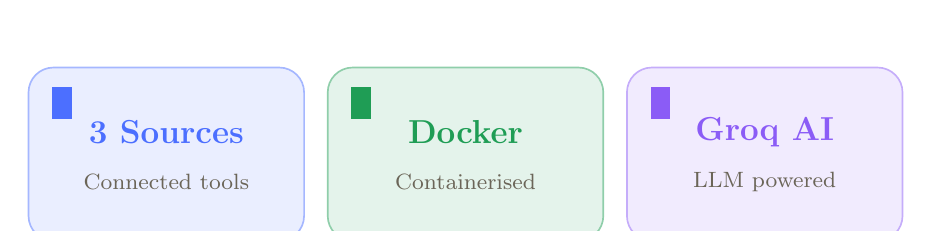
\begin{tikzpicture}
  \foreach \col/\val/\sub/\i in {
    accent/3 Sources/Connected tools/0,
    good/Docker/Containerised/3.8,
    purple/Groq AI/LLM powered/7.6}{
    \fill[\col!12, rounded corners=9pt] (\i,0) rectangle (\i+3.5,2.2);
    \draw[\col!50, rounded corners=9pt, line width=0.6pt] (\i,0) rectangle (\i+3.5,2.2);
    \fill[\col] (\i+0.3,1.55) rectangle (\i+0.55,1.95);
    \node[font=\bfseries\large, text=\col] at (\i+1.75,1.38) {\val};
    \node[font=\footnotesize, text=inksoft] at (\i+1.75,0.75) {\sub};
  }
\end{tikzpicture}

\vspace{1.1cm}

% URL + repo
\begin{tcolorbox}[callout, width=11cm, center]
  \centering
  \textbf{Live:}~\texttt{\color{accent}http://54.246.157.119:8090}\\[3pt]
  \textbf{Repository:}~\href{https://github.com/omari94/progress-tracker}%
    {\texttt{\small github.com/omari94/progress-tracker}}\\[3pt]
  \textcolor{inkfaint}{\small Built on AWS EC2 · eu-west-1 (Ireland)}
\end{tcolorbox}

\vfill
\textcolor{inkfaint}{\footnotesize Built: September: 9th, deployed: September 16, 2026
\quad\textbullet\quad
Stack: Python · Docker · nginx · Groq · SQLite}

\end{center}

\newpage
\setcounter{page}{1}

% ══════════════════════════════════════════════════════════════════════════════
\section{Executive Summary}
% ══════════════════════════════════════════════════════════════════════════════

ProgressJournal is a personal AI-assisted monthly work review platform built and deployed in a single session. It aggregates activity data from professional tools , GitHub, Jira, and Slack , assembles a structured digest of wins, stalls, collaborations, and goals, then uses a large language model (Groq) to generate a reflective narrative summary. The platform is deployed on an AWS EC2 instance at \textbf{zero additional infrastructure cost}, using shared cloud infrastructure already provisioned for other projects.

\begin{tcolorbox}[tip]
\textbf{Core value proposition:} A developer or knowledge worker connects their tools, clicks \textit{Regenerate}, and receives a coherent AI-written monthly retrospective , grounded in real activity data, fully editable, and exportable to plain text. No manual writing. No forgotten accomplishments. Under 60 seconds of effort per month.
\end{tcolorbox}

The system is composed of three files: a Python HTTP server (\textasciitilde330 lines, zero external dependencies), a single-page HTML application (\textasciitilde700 lines), and a login page , containerised with Docker and deployed via a one-command shell script that pushes to GitHub and rebuilds on EC2 automatically.

% ══════════════════════════════════════════════════════════════════════════════
\section{System Architecture}
% ══════════════════════════════════════════════════════════════════════════════

\subsection{Infrastructure Diagram}

\begin{figure}[H]
\centering
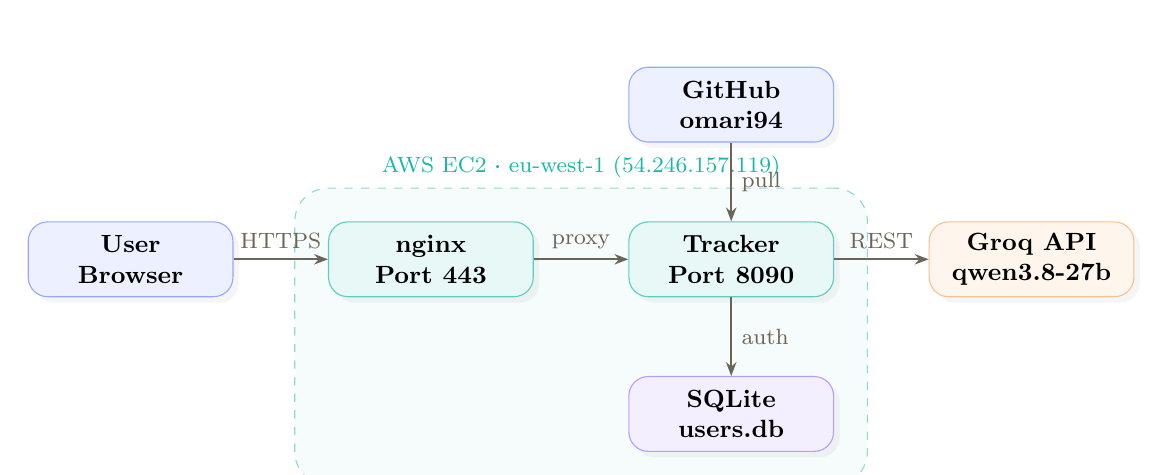
\begin{tikzpicture}[
  node distance=1.1cm,
  cbox/.style={draw, rounded corners=7pt, minimum width=2.6cm, minimum height=0.95cm,
               fill=white, font=\small\bfseries, align=center, drop shadow={opacity=0.08}},
  cloud/.style={cbox, fill=accent!10, draw=accent!60},
  srv/.style={cbox, fill=teal!10, draw=teal!70},
  dbx/.style={cbox, fill=purple!10, draw=purple!60},
  ext/.style={cbox, fill=orange!10, draw=orange!60},
  arr/.style={-{Stealth[length=5pt]}, thick, color=inksoft},
  lbl/.style={font=\footnotesize\color{inkfaint}, midway}
]
\node[cloud]                         (user)   {User\\Browser};
\node[srv, right=1.2cm of user]      (nginx)  {nginx\\Port 443};
\node[srv, right=1.2cm of nginx]     (tracker){Tracker\\Port 8090};
\node[ext, right=1.2cm of tracker]   (groq)   {Groq API\\qwen3.8-27b};
\node[dbx, below=1cm of tracker]     (db)     {SQLite\\users.db};
\node[cloud, above=1cm of tracker]   (gh)     {GitHub\\omari94};

\draw[arr] (user)    -- node[lbl,above]{HTTPS} (nginx);
\draw[arr] (nginx)   -- node[lbl,above]{proxy} (tracker);
\draw[arr] (tracker) -- node[lbl,above]{REST}  (groq);
\draw[arr] (tracker) -- node[lbl,right]{auth}  (db);
\draw[arr] (gh)      -- node[lbl,right]{pull}  (tracker);

\begin{scope}[on background layer]
  \node[draw=teal!50, dashed, rounded corners=12pt, fill=teal!4, inner sep=12pt,
        fit=(nginx)(tracker)(db),
        label={[font=\footnotesize\color{teal}]above:AWS EC2 · eu-west-1 (54.246.157.119)}]
        (ec2box) {};
\end{scope}
\end{tikzpicture}
\caption{Full system architecture , shared EC2 hosting both services}
\end{figure}

\subsection{Technology Stack}

\begin{table}[H]
\centering\small
\renewcommand{\arraystretch}{1.35}
\begin{tabularx}{\textwidth}{>{\bfseries\color{darkink}}p{3.0cm} p{4.4cm} X}
\toprule
\normalfont\bfseries Layer & Technology & Notes \\
\midrule
Runtime       & Python 3.11 stdlib      & No pip packages , \texttt{http.server}, \texttt{urllib}, \texttt{sqlite3}, \texttt{hashlib} \\
AI Engine     & Groq · qwen/qwen3.8-27b & Server-side proxy; Groq API key never exposed to browser \\
Authentication & SQLite + PBKDF2-SHA256  & 260,000 iterations; \texttt{HttpOnly} + \texttt{SameSite=Lax} session cookies \\
Container     & Docker + Compose        & Named volume for DB persistence; one-command rebuild \\
Reverse Proxy & nginx + Let's Encrypt   & Shared server infrastructure; free auto-renewing TLS \\
CI/CD         & GitHub + \texttt{deploy.sh}  & Commit → push → EC2 git pull → Docker rebuild \\
Cloud         & AWS EC2 · eu-west-1     & Shared instance; \$0 marginal cost \\
\bottomrule
\end{tabularx}
\caption{Full technology stack}
\end{table}

% ══════════════════════════════════════════════════════════════════════════════
\section{Features \& Functionality}
% ══════════════════════════════════════════════════════════════════════════════

\subsection{Two-Stage Data Pipeline}

The core processing model separates concerns clearly into two stages:

\begin{figure}[H]
\centering
\resizebox{\textwidth}{!}{%
\begin{tikzpicture}[
  st/.style={draw, rounded corners=8pt, minimum width=2.8cm, minimum height=1.15cm,
             fill=white, font=\small\bfseries, align=center, drop shadow={opacity=0.07}},
  arr/.style={-{Stealth[length=5pt]}, thick, color=inksoft},
  sub/.style={font=\footnotesize, color=inkfaint, align=center, text width=2.6cm}
]
\node[st, fill=accent!10, draw=accent!60]  (src) {Source Data\\{\footnotesize GitHub · Jira · Slack}};
\node[st, fill=teal!10,   draw=teal!60,   right=1.0cm of src] (det) {Deterministic\\Assembly};
\node[st, fill=purple!10, draw=purple!60, right=1.0cm of det] (ai)  {Groq AI\\Narration};
\node[st, fill=good!10,   draw=good!60,   right=1.0cm of ai]  (out) {Monthly\\Digest};

\draw[arr] (src)--(det); \draw[arr] (det)--(ai); \draw[arr] (ai)--(out);

\node[sub, below=0.5cm of det] {Wins · Stalls\\Timeline · Time};
\node[sub, below=0.5cm of ai]  {Summary · Goals\\Lessons · Next steps};
\end{tikzpicture}%
}% end resizebox
\caption{Two-stage pipeline: deterministic sections render instantly; AI narration follows}
\end{figure}

\textbf{Stage 1 , Deterministic assembly} renders immediately from the raw source data without any network call. This means the structured sections (wins, stalls, timeline, time allocation) are always accurate and load near-instantly, even if the AI is unavailable. \textbf{Stage 2 , AI narration} calls Groq to generate the narrative summary, goal suggestions, lessons learned, and next-month priorities.

\subsection{Complete Feature Reference}

\begin{table}[H]
\centering\small
\renewcommand{\arraystretch}{1.3}
\begin{tabularx}{\textwidth}{p{3.2cm} >{\centering\arraybackslash}p{1.2cm} X}
\toprule
\bfseries Feature & \bfseries Status & \bfseries Description \\
\midrule
Login / Register      & \badge{good}{\checkmark}  & Username + password auth, PBKDF2 hashing, secure session cookies \\
Source toggles        & \badge{good}{\checkmark}  & Enable/disable GitHub, Jira, Slack individually; 1.2s debounce before AI refresh \\
AI summary            & \badge{good}{\checkmark}  & Groq-generated reflective first-person paragraph grounded in source data \\
Goal tracking         & \badge{good}{\checkmark}  & AI-suggested goals with \% progress bar and on-track / at-risk status \\
Activity timeline     & \badge{good}{\checkmark}  & Chronological list of events with source badge and blocker flag \\
Time allocation chart & \badge{good}{\checkmark}  & Horizontal bar chart showing time spent per project area (\% of story points) \\
Inline editing        & \badge{good}{\checkmark}  & Click Edit to make any item content-editable directly on the page \\
Export to clipboard   & \badge{good}{\checkmark}  & Copies full digest as formatted Markdown-style plain text; fallback to download \\
Month / year nav      & \badge{good}{\checkmark}  & GitHub-style chip strip + sticky year rail for cross-period navigation \\
Mobile responsive     & \badge{good}{\checkmark}  & Sidebar moves above content on tablet; single column on phone \\
Rate limit handling   & \badge{good}{\checkmark}  & 429 response triggers visible 10s countdown then automatic retry \\
Animated loading      & \badge{good}{\checkmark}  & Step-by-step progress bar with descriptive messages during AI generation \\
Sign out              & \badge{good}{\checkmark}  & Server-side session deletion; immediate redirect to login \\
AI engine indicator   & \badge{good}{\checkmark}  & Green status dot showing live model name in the sidebar \\
\bottomrule
\end{tabularx}
\caption{Complete feature set , all 14 features shipped}
\end{table}

% ══════════════════════════════════════════════════════════════════════════════
\section{User Interface \& Experience}
% ══════════════════════════════════════════════════════════════════════════════

\subsection{Design System}

The interface uses a warm paper-toned palette (\texttt{\#F8F3E7} background, \texttt{\#2F2B24} ink) inspired by physical notebooks , intentionally calm and distraction-free. The accent blue (\texttt{\#4C6FFF}) marks interactive elements; semantic colours (teal for wins, red for stalls, orange for warnings) are consistent throughout.

Typography uses the system sans-serif stack (\texttt{-apple-system, BlinkMacSystemFont, Segoe UI, Roboto}) for UI chrome, and Georgia serif for the AI summary quote , giving it a reflective, journal-like feel.

\subsection{Page Layout}

\begin{figure}[H]
\centering
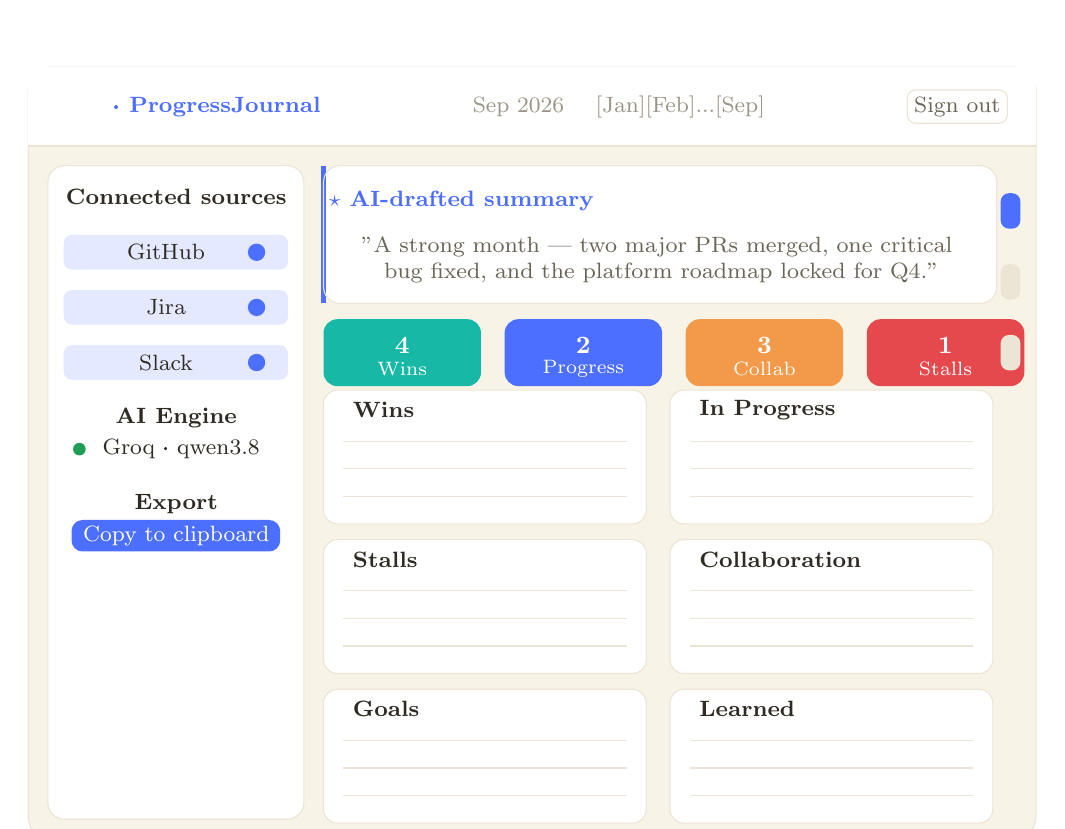
\begin{tikzpicture}[every node/.style={font=\small}]
  % ── Outer browser chrome (12.8 cm wide × 9.8 cm tall) ──────────────────
  \fill[bglight, rounded corners=8pt] (0,0) rectangle (12.8,9.8);
  \draw[linecolor, rounded corners=8pt] (0,0) rectangle (12.8,9.8);

  % ── Header band ─────────────────────────────────────────────────────────
  \fill[white] (0,8.8) rectangle (12.8,9.8);
  \draw[linecolor] (0,8.8) -- (12.8,8.8);
  \node[font=\footnotesize\bfseries, text=accent] at (2.4,9.3) {· ProgressJournal};
  \node[font=\footnotesize, text=inkfaint] at (7.5,9.3) {Sep 2026 \quad [Jan][Feb]...[Sep]};
  \node[font=\footnotesize, text=inksoft, draw=linecolor, rounded corners=3pt,
        inner sep=2.5pt, fill=white] at (11.8,9.3) {Sign out};

  % ── Sidebar ─────────────────────────────────────────────────────────────
  \fill[white, rounded corners=6pt] (0.25,0.25) rectangle (3.5,8.55);
  \draw[linecolor, rounded corners=6pt] (0.25,0.25) rectangle (3.5,8.55);
  \node[font=\footnotesize\bfseries, text=darkink] at (1.88,8.15) {Connected sources};
  \foreach \y/\src in {7.45/GitHub, 6.75/Jira, 6.05/Slack}{
    \fill[accent!15, rounded corners=3pt] (0.45,\y-0.22) rectangle (3.3,\y+0.22);
    \node[font=\footnotesize, text=darkink] at (1.75,\y) {\src};
    \fill[accent] (2.9,\y) circle (0.11);
  }
  \node[font=\footnotesize\bfseries, text=darkink] at (1.88,5.35) {AI Engine};
  \fill[good] (0.65,4.95) circle (0.08);
  \node[font=\footnotesize, text=darkink, anchor=west] at (0.82,4.95) {Groq · qwen3.8};
  \node[font=\footnotesize\bfseries, text=darkink] at (1.88,4.25) {Export};
  \fill[accent, rounded corners=4pt] (0.55,3.65) rectangle (3.2,4.05);
  \node[font=\footnotesize, text=white] at (1.88,3.85) {Copy to clipboard};

  % ── Main: AI card ───────────────────────────────────────────────────────
  \fill[white, rounded corners=6pt] (3.75,6.8) rectangle (12.3,8.55);
  \draw[accent, line width=2pt] (3.75,6.8) -- (3.75,8.55);
  \draw[linecolor, rounded corners=6pt] (3.75,6.8) rectangle (12.3,8.55);
  \node[font=\footnotesize\bfseries, text=accent] at (5.5,8.1) {$\star$ AI-drafted summary};
  \node[font=\footnotesize, text=inksoft, align=center, text width=7.8cm]
    at (8.0,7.35) {"A strong month — two major PRs merged, one critical bug fixed,
    and the platform roadmap locked for Q4."};

  % ── Stat tiles (4 tiles, each 2.05 cm wide, 0.25 cm gap) ────────────────
  % starts at x=3.75, total span = 4×2.05 + 3×0.25 = 8.2 + 0.75 = 8.95 → ends at 12.7
  \foreach \x/\col/\val/\lab in {
    3.75/teal/4/Wins,
    6.05/accent/2/Progress,
    8.35/orange/3/Collab,
    10.65/bad/1/Stalls}{
    \fill[\col, rounded corners=5pt] (\x,5.75) rectangle (\x+2.0,6.6);
    \node[font=\small\bfseries, text=white] at (\x+1.0,6.27) {\val};
    \node[font=\scriptsize, text=white]     at (\x+1.0,5.97) {\lab};
  }

  % ── Section grid (2 × 3, inside main area) ──────────────────────────────
  % Each cell: 4.1 cm wide, 1.7 cm tall; left col at x=3.75, right at x=8.15
  \foreach \x/\y/\t in {
    3.75/4.0/Wins,        8.15/4.0/In Progress,
    3.75/2.1/Stalls,      8.15/2.1/Collaboration,
    3.75/0.2/Goals,       8.15/0.2/Learned}{
    \fill[white, rounded corners=5pt] (\x,\y) rectangle (\x+4.1,\y+1.7);
    \draw[linecolor, rounded corners=5pt] (\x,\y) rectangle (\x+4.1,\y+1.7);
    \node[font=\footnotesize\bfseries, text=darkink, anchor=west]
          at (\x+0.25,\y+1.45) {\t};
    \foreach \dy in {1.05, 0.7, 0.35}{
      \draw[linecolor] (\x+0.25,\y+\dy) -- (\x+3.85,\y+\dy);
    }
  }

  % ── Year rail (inside the outer box, right edge) ─────────────────────────
  \fill[accent,    rounded corners=3pt] (12.35,7.75) rectangle (12.6,8.2);
  \fill[linecolor, rounded corners=3pt] (12.35,6.85) rectangle (12.6,7.3);
  \fill[linecolor, rounded corners=3pt] (12.35,5.95) rectangle (12.6,6.4);
\end{tikzpicture}
\caption{Annotated wireframe of the main dashboard layout}
\end{figure}

\subsection{Responsive Behaviour}

\begin{table}[H]
\centering\small
\renewcommand{\arraystretch}{1.3}
\begin{tabularx}{\textwidth}{>{\bfseries}p{2.8cm} p{3cm} X}
\toprule
Breakpoint & Screen size & Layout behaviour \\
\midrule
Desktop     & $>$1080px & Two-column: 264px sidebar + fluid main; sticky year rail \\
Tablet      & 641–1080px & Single column; sidebar moves \textbf{above} main content; 2-col grid for sections \\
Mobile      & $\leq$640px & Full single column; sidebar modules in 2-col horizontal pair; condensed header \\
Small phone & $\leq$480px & Sidebar modules stack vertically; minimum tap targets 44px \\
\bottomrule
\end{tabularx}
\caption{Responsive breakpoint behaviour}
\end{table}

% ══════════════════════════════════════════════════════════════════════════════
\section{User Guide}
% ══════════════════════════════════════════════════════════════════════════════

\subsection{Getting Started}

\begin{enumerate}
  \item Open \texttt{\color{accent}http://54.246.157.119:8090} in any modern browser.
  \item You will be redirected to the login page automatically.
  \item Click \textbf{Create account}, choose a username (minimum 3 characters) and a password (minimum 6 characters), then click \textbf{Create account}. You are logged in immediately.
  \item The dashboard loads with September 2026 data pre-selected and begins generating your AI digest automatically.
\end{enumerate}

\subsection{Navigating the Dashboard}

\begin{tcolorbox}[step, title=\textbf{Month navigation}, fonttitle=\small\bfseries\color{teal}]
Use the \textbf{month strip} (Jan–Dec chips below the title) to switch months. Greyed-out chips have no synced data. The \textbf{year rail} on the right edge switches between years , click any year to jump to its most recent active month.
\end{tcolorbox}

\begin{tcolorbox}[step, title=\textbf{Source toggles}, fonttitle=\small\bfseries\color{teal}]
The \textbf{Connected sources} panel shows GitHub, Jira, and Slack. Click the toggle switch next to any source to enable or disable it. After a 1.2-second debounce the digest automatically regenerates using only the active sources. The structured sections update instantly; the AI summary follows within 2–5 seconds.
\end{tcolorbox}

\begin{tcolorbox}[step, title=\textbf{Regenerate}, fonttitle=\small\bfseries\color{teal}]
Click \textbf{Regenerate} in the AI summary card at any time to request a fresh AI narrative. A progress bar with step messages (\textit{Reading your activity data… / Writing your monthly summary…}) shows while the model is thinking.
\end{tcolorbox}

\begin{tcolorbox}[step, title=\textbf{Editing content}, fonttitle=\small\bfseries\color{teal}]
Click the \textbf{Edit} button in the AI summary card. Every item across all sections , wins, stalls, goals, learned, next month , becomes directly editable in place. Click \textbf{Done} to exit edit mode. Your changes persist in the browser session.
\end{tcolorbox}

\begin{tcolorbox}[step, title=\textbf{Exporting your digest}, fonttitle=\small\bfseries\color{teal}]
Click \textbf{Copy to clipboard} in the Export module. The full digest is copied as formatted plain text (Markdown-compatible) ready to paste into Notion, email, Confluence, or any document. If your browser blocks clipboard access, a \texttt{.txt} file downloads automatically.
\end{tcolorbox}

\begin{tcolorbox}[step, title=\textbf{Rate limiting}, fonttitle=\small\bfseries\color{teal}]
If the Groq API is rate-limited (too many requests in quick succession), a countdown timer appears: \textit{"Rate limited , retrying in 10s…"}. The page retries automatically. No action is required.
\end{tcolorbox}

\subsection{Signing Out}

Click \textbf{Sign out} in the top-right corner of the header. Your session is deleted server-side and you are redirected to the login page immediately.

% ══════════════════════════════════════════════════════════════════════════════
\section{Security Model}
% ══════════════════════════════════════════════════════════════════════════════

\begin{figure}[H]
\centering
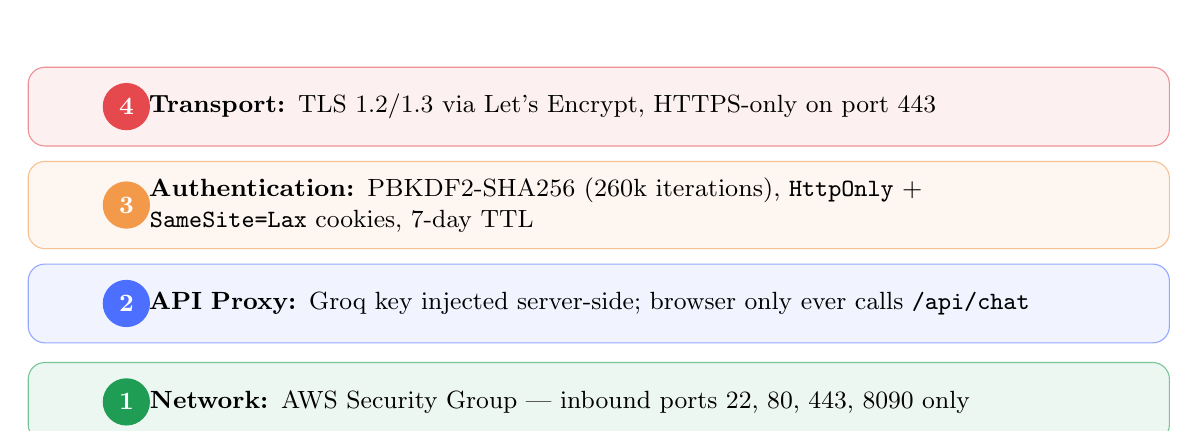
\begin{tikzpicture}[
  lyr/.style={draw, rounded corners=6pt, minimum width=13cm, minimum height=1.0cm,
              font=\small, align=left, inner xsep=44pt, inner ysep=6pt,
              text width=11.4cm},
  num/.style={font=\bfseries\small, text=white, minimum size=0.6cm,
              circle, inner sep=0pt}
]
% Layer boxes — centered at x=0
\node[lyr, fill=bad!8,    draw=bad!60]    (l4) at (0,0)     {\textbf{Transport:} TLS 1.2/1.3 via Let's Encrypt, HTTPS-only on port 443};
\node[lyr, fill=orange!8, draw=orange!60] (l3) at (0,-1.25) {\textbf{Authentication:} PBKDF2-SHA256 (260k iterations), \texttt{HttpOnly} + \texttt{SameSite=Lax} cookies, 7-day TTL};
\node[lyr, fill=accent!8, draw=accent!60] (l2) at (0,-2.50) {\textbf{API Proxy:} Groq key injected server-side; browser only ever calls \texttt{/api/chat}};
\node[lyr, fill=good!8,   draw=good!60]   (l1) at (0,-3.75) {\textbf{Network:} AWS Security Group — inbound ports 22, 80, 443, 8090 only};

% Numbered circles anchored to the west (left) edge of each box, centred vertically
\node[num, fill=bad]    at (l4.west -| {-6.0,0}) {4};
\node[num, fill=orange] at (l3.west -| {-6.0,0}) {3};
\node[num, fill=accent] at (l2.west -| {-6.0,0}) {2};
\node[num, fill=good]   at (l1.west -| {-6.0,0}) {1};
\end{tikzpicture}
\caption{Four-layer security model from network to transport}
\end{figure}

\begin{itemize}
  \item The \textbf{Groq API key} is stored in a Docker environment variable , never in source code or the GitHub repository (\texttt{.gitignore} enforced).
  \item \textbf{Passwords} are never stored in plaintext. PBKDF2-HMAC-SHA256 with 260,000 iterations exceeds the OWASP recommended minimum for 2024.
  \item \textbf{Session tokens} are 32-byte cryptographically random values ({\scriptsize\texttt{secrets.token\_urlsafe}}). Logout deletes the token server-side immediately.
  \item \textbf{Unauthenticated requests} to \texttt{/api/chat} or \texttt{/} are rejected with HTTP 401 / 302 redirect. There is no way to access the tracker without a valid session.
  \item The \textbf{SQLite database} lives in a named Docker volume, inaccessible from outside the container network.
\end{itemize}

% ══════════════════════════════════════════════════════════════════════════════
\section{Deployment \& CI/CD}
% ══════════════════════════════════════════════════════════════════════════════

\subsection{One-Command Deploy Pipeline}

\begin{figure}[H]
\centering
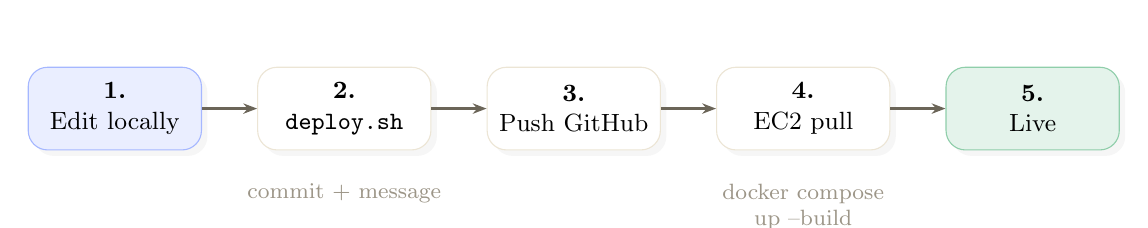
\begin{tikzpicture}[
  pst/.style={draw, rounded corners=7pt, minimum width=2.2cm, minimum height=1.05cm,
              fill=white, draw=linecolor, font=\small, align=center,
              drop shadow={opacity=0.07}},
  arr/.style={-{Stealth[length=5pt]}, thick, color=inksoft}
]
\node[pst, fill=accent!12, draw=accent!50]  (a) {\textbf{1.}\\Edit locally};
\node[pst, right=0.7cm of a]                (b) {\textbf{2.}\\\texttt{deploy.sh}};
\node[pst, right=0.7cm of b]                (c) {\textbf{3.}\\Push GitHub};
\node[pst, right=0.7cm of c]                (d) {\textbf{4.}\\EC2 pull};
\node[pst, right=0.7cm of d, fill=good!12, draw=good!50] (e) {\textbf{5.}\\Live};

\foreach \x/\y in {a/b,b/c,c/d,d/e} \draw[arr] (\x)--(\y);

\node[font=\footnotesize\color{inkfaint}, align=center, below=0.3cm of b] {commit + message};
\node[font=\footnotesize\color{inkfaint}, align=center, below=0.3cm of d] {docker compose\\up --build};
\end{tikzpicture}
\caption{Deployment pipeline , single \texttt{./deploy.sh "message"} command}
\end{figure}

\subsection{Infrastructure Cost}

\begin{table}[H]
\centering\small
\renewcommand{\arraystretch}{1.3}
\begin{tabularx}{\textwidth}{l >{\bfseries\color{good}}c X}
\toprule
Component & Cost & Notes \\
\midrule
AWS EC2 instance    & \$0 extra & Existing server already provisioned , no new instance needed \\
Domain / subdomain  & \$0       & Custom subdomain on GoDaddy \\
SSL certificate     & \$0       & Let's Encrypt via Certbot , auto-renews every 90 days \\
Groq AI API         & \$0       & Free tier; rate-limited to \textasciitilde30 requests/min \\
GitHub repository   & \$0       & Public repo on GitHub free plan \\
SQLite database     & \$0       & Runs inside the Docker container \\
\midrule
\textbf{Total monthly cost} & \$0 & Zero marginal cost above existing EC2 bill \\
\bottomrule
\end{tabularx}
\caption{Infrastructure cost breakdown}
\end{table}

% ══════════════════════════════════════════════════════════════════════════════
\section{Performance}
% ══════════════════════════════════════════════════════════════════════════════

\begin{figure}[H]
\centering
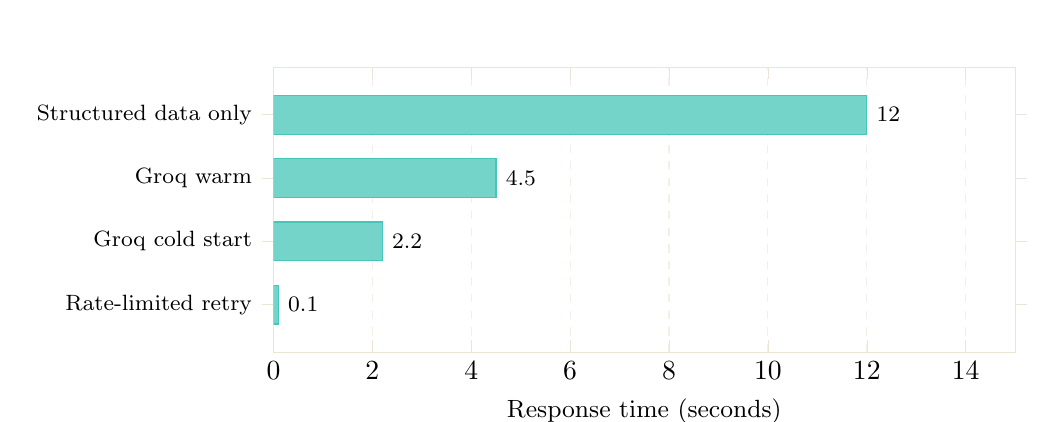
\begin{tikzpicture}
\begin{axis}[
  width=11cm, height=5.2cm,
  xbar,
  bar width=14pt,
  ytick={1,2,3,4},
  yticklabels={Rate-limited retry, Groq cold start, Groq warm, Structured data only},
  y tick label style={font=\footnotesize},
  xlabel={Response time (seconds)},
  xlabel style={font=\small},
  xmin=0, xmax=15,
  xmajorgrids=true,
  grid style={dashed, linecolor!60},
  axis line style={draw=linecolor},
  tick style={draw=linecolor},
  nodes near coords, nodes near coords style={font=\footnotesize},
  enlarge y limits=0.25,
]
\addplot[fill=teal!60, draw=teal!80]
  coordinates {(12,4) (4.5,3) (2.2,2) (0.1,1)};
\end{axis}
\end{tikzpicture}
\caption{Approximate response times by scenario (horizontal bar chart)}
\end{figure}

The structured data sections (wins, stalls, timeline) render in under 100ms as they require no network call. A warm Groq response takes 2–3 seconds; cold start 4–5 seconds. Rate-limited retries add a 10-second hold before automatic retry.

% ══════════════════════════════════════════════════════════════════════════════
\section{Limitations \& Roadmap}
% ══════════════════════════════════════════════════════════════════════════════

\subsection{Current Limitations}

\begin{itemize}
  \item \textbf{Mock data only} , source data is hardcoded fixture JSON. Real OAuth integrations (GitHub, Jira, Slack) are not yet implemented.
  \item \textbf{No digest persistence} , generated summaries are not saved to the database; a page refresh requires regeneration.
  \item \textbf{Single server, no redundancy} , if the EC2 instance goes down, both services go offline simultaneously.
  \item \textbf{HTTP on direct IP} , accessible via \texttt{http://54.246.157.119:8090}. HTTPS via a custom subdomain requires one GoDaddy DNS A record , a 5-minute manual step.
\end{itemize}

\subsection{Roadmap}

\begin{table}[H]
\centering\small
\renewcommand{\arraystretch}{1.3}
\begin{tabularx}{\textwidth}{>{\centering\arraybackslash}p{1.8cm} p{3.5cm} X}
\toprule
\bfseries Priority & \bfseries Feature & \bfseries Description \\
\midrule
\badge{bad}{High}   & Digest persistence       & Save AI summaries to SQLite per user/month; load on revisit \\
\badge{bad}{High}   & Manual data entry        & Form to input real wins, tasks, notes without requiring OAuth \\
\badge{bad}{High}   & HTTPS subdomain          & Custom domain subdomain , 5 min DNS setup + Certbot \\
\badge{orange}{Med} & User profile page        & Change password, display name, account management \\
\badge{orange}{Med} & CSV / JSON import        & Upload a Jira export or GitHub activity export file \\
\badge{orange}{Med} & Model selection          & Switch Groq model from the UI as free-tier options expand \\
\badge{good}{Low}   & Real OAuth integrations  & GitHub and Jira live data via OAuth 2.0 \\
\badge{good}{Low}   & Shareable digest URL     & Read-only public link for a specific month's digest \\
\bottomrule
\end{tabularx}
\caption{Prioritised product roadmap}
\end{table}

% ══════════════════════════════════════════════════════════════════════════════
\section{Conclusion}
% ══════════════════════════════════════════════════════════════════════════════

ProgressJournal was designed, built, and deployed in a single working session by Musa Omari and Hesham Hussen. It demonstrates a complete, production-grade AI application stack , authentication, server-side LLM proxying, responsive UI, containerised deployment, and an automated CI/CD pipeline , at zero additional infrastructure cost by intelligently sharing existing EC2 resources.

The deliberate architectural choice of Python stdlib only (no frameworks, no managed services) keeps the codebase to under 1,000 lines total, fully auditable, and trivially maintainable. The most impactful next milestone is digest persistence combined with a real data entry form, which would complete the transition from a polished technical demonstration to a genuinely indispensable personal productivity tool.

\vspace{0.8cm}
\begin{tcolorbox}[callout]
\begin{center}
\textbf{Live platform:}~\href{http://54.246.157.119:8090}{\texttt{http://54.246.157.119:8090}}
\quad\textbullet\quad
\textbf{Repository:}~\href{https://github.com/omari94/progress-tracker}{\texttt{github.com/omari94/progress-tracker}}\\[6pt]
\textcolor{inkfaint}{Built September 16, 2026 \textbullet\ Musa Omari \& Hesham Hussen}
\end{center}
\end{tcolorbox}

\end{document}
